% This file is part of the stream_information project.
% Copyright 2017 the authors. All rights reserved.

% # style notes
% - it is Cram\'er--Rao not Cram\'er-Rao. And yet Fisher-matrix not Fisher--matrix.

% TODO:
% - Reference for the dustmaps package? See software section.

% Story:
% - progenitor - show std_v, std_phi2
% - 2 gaps, 1 under-density - epicycles/streakline? percentiles in polynomial
% - spur - encounter?

\documentclass[modern]{aastex62}

\usepackage{amsmath}

% typography
\setlength{\parindent}{1.\baselineskip}
\newcommand{\acronym}[1]{{\small{#1}}}
\newcommand{\package}[1]{\textsl{#1}}
\newcommand{\gaia}{\textsl{Gaia}}
\newcommand{\pans}{\textsl{Pan-STARRS}}
\newcommand{\DR}{\acronym{DR2}}
\newcommand{\msun}{\textrm{M}_\odot}
\newcommand{\kpc}{\textrm{kpc}}
\newcommand{\feh}{\ensuremath{[\textrm{Fe} / \textrm{H}]}}
\newcommand{\article}{\textsl{Letter}}

% aastex parameters
% \received{not yet; THIS IS A DRAFT}
%\revised{not yet}
%\accepted{not yet}
% % Adds "Submitted to " the arguement.
% \submitjournal{ApJ}
\shorttitle{GD-1 in Gaia DR2}
\shortauthors{Price-Whelan \& Bonaca}

%@arxiver{}

\begin{document}\sloppy\sloppypar\raggedbottom\frenchspacing % trust me

\title{Off the beaten path: \\
       ...}
% Gaia DR2 reveals stream stars...
% A first look at the GD-1 stellar stream with Gaia DR2

\author[0000-0003-0872-7098]{Adrian~M.~Price-Whelan}
\affiliation{Department of Astrophysical Sciences,
             Princeton University, Princeton, NJ 08544, USA}
\email{adrn@astro.princeton.edu}
\correspondingauthor{Adrian M. Price-Whelan}

\author[0000-0002-7846-9787]{Ana Bonaca}
\affil{Harvard--Smithsonian Center for Astrophysics, Cambridge, MA 02138, USA}


\begin{abstract}\noindent % trust me
Tidally-disrupted globular clusters are transformed into thin, dynamically-cold
streams of stars that are extremely valuable tracers of the large- and
small-scale distribution of matter in the Galaxy.
Most stellar streams discovered around the Milky Way reside in the Galactic halo
and are therefore primarily sensitive to the distribution of dark matter.
We present a sample of highly-probable members of the longest cold stream, GD-1,
selected to have small parallaxes and retrograde proper motions using data from
the \gaia\ mission, and \pans\ photometry consistent with an old and metal-poor
population at a distance of $\sim10~\kpc$.
This selection extended the stream by $10^\circ$(?), revealed a possible location of the progenitor and mapped significant density variations along the stream in unprecedented detail.
In addition to several prominent gaps, for the first time we also find evidence of stream members off the main track.
No(?) secular formation mechanisms predict the existence of such spurs, but they are a natural result of a stream interaction with a massive perturber.
Based on the impulse approximation arguments, we estimate that the detected underdensity and the associated spur could have been induced by a perturbation of a $\sim10^7\,\rm M_\odot$(?) object $\sim 0.5\,$Gyr ago.
Our model of GD-1 indicates that the stream crosses the Galactic plane at a large radius, which puts the likely origin of the perturber beyond the stellar disk.
\end{abstract}

\keywords{Galaxy: halo --- dark matter}

\section{Introduction}
\label{sec:intro}

Dynamically cold stellar streams are formed from the tidal disruption of stellar
systems by the gravitational field of their host galaxy.
The phase-space density and mean track of stars in streams therefore encode
information about the underlying distribution and shape of mass on galactic
scales (e.g., \citealt{Johnston:1999, Bonaca:2018}).
Most stellar streams are found in the halos of galaxies and are therefore
important tracers of the large-scale distribution of dark matter in galactic
halos.

Long, thin stellar streams are also excellent laboratories for studying
small-scale structures in the mass distribution:
thin streams can remain coherent for tens of orbital periods, depending in
detail on the symmetries of the underlying galactic mass distribution (e.g.,
\citealt{Erkal:2016}).
Encounters between massive perturbers and stream stars imprint variations in the
phase-space density that can persist and remain visible for close to their total
survival time (e.g., \citealt{Yoon:2011}).
In this sense, streams represent one of the most promising directions for
studying or ruling out the existence of small-scale dark matter sub-halos, as
would be predicted by standard $\Lambda$ Cold Dark Matter ($\Lambda$CDM) theory
(\citealt{Erkal:2015, Sanders:2016, Bovy:2017}).

Over 30 candidate stellar streams have been discovered throughout the halo of
the Milky Way, thanks to large-area, multi-band photometric surveys (especially
the Sloan Digital Sky Survey, SDSS; \citealt{York:2000}).
The Milky Way streams have a wide range of properties such as length, velocity
dispersion, and density (e.g., \citealt{Odenkirchen:2001, Grillmair:2006,
Grillmair:2006b, Belokurov:2006, Belokurov:2007, Bonaca:2012, Shipp:2018}; see
also the recent review \citealt{Grillmair:2016, Newberg:2016}), and the majority
have no obvious, bound progenitor systems;
of the thin, likely globular-cluster-origin streams, only two have clear
progenitors (NGC 5466 and Palomar 5).

The most prominent and longest (in angular extent) thin stream is the GD-1
stream, named after its discoverers (\citealt{Grillmair:2006}).
GD-1 was found using a matched filter on photometric data from the SDSS and
spans over $60^\circ$ in Heliocentric sky coordinates, partially because of its
relative closeness to the sun ($\approx 7$--$10~\textrm{kpc}$).
Despite its proximity, no remnant progenitor cluster or stellar system has been
found associated with the stream, but its metallicity ($\feh \approx -1.4$;
\citealt{Koposov:2010}) and estimated stellar mass ($M \approx 2 \times
10^4~\msun$; \citealt{Koposov:2010}) are consistent with being a disrupted
globular cluster.

The long physical length of the GD-1 stream ($\sim 15~\kpc$) and location in the
Galactic halo (pericentric distance $r_\textrm{peri} \sim 13~\kpc$) make it an
ideal object for constraining the gravitational potential of dark matter in the
inner Milky Way.
Indeed, both from fitting orbits to binned phase-space measurements along the
GD-1 stream (\citealt{Koposov:2010}) and from modeling the stream track in
phase-space coordinates (\citealt{Bovy:2016}), it has been shown that the dark
matter distribution within its orbit is consistent with or nearly spherical.

Its long length --- and therefore its implied old dynamical age --- combined
with its particular orbit also make it a prime stream to search for interactions
with dark matter subhalos:
because of its large pericentric distance and retrograde orbit with respect to
the Galactic bar, density variations in the stream are not expected from either
interactions with giant molecular clouds (\citealt{Amorisco:2016}) or resonant
encounters with the bar (\citealt{Pearson:2017}).
By assuming an age [...], \citet{Erkal:2016} predict that XX (~1 gap??).

From SDSS photometry, hints of further gaps and under-densities have been
identified in the GD-1 stream, but with low significance
(\citealt{Carlberg:2013}).
More recently, deep photometry of GD-1 from CFHT/Megacam has revealed
interesting small-scale ``wiggles'' and significant density variations along a $\approx 45^\citc$ span of the stream (\citealt{DeBoer:2017}):
[summarize their conclusions].

In this \article, we present clearest view of the GD-1 stream to date using
astrometric data from the \gaia\ mission data release 2 (\DR) combined with
precise photometry from the \pans\ survey.
We find XX under-densities gaps, some consistent with ...
We revisit...do not try to model or fit for Galactic potential.
Focus on stream properties, data.

\section{Data}
\label{sec:data}

- Transform to GD-1 coordinates (Koposov et al.)
    - Can see deviation from great circle
- Cut to be close to latitude = 0
- Cut to get proper motion over-density
- Color-magnitude filtering

Comment on these here - add figure for both in Appendix?
- Dust / no significant extinction - combine with other figure
- Scanning pattern - just discuss, no figure

Most of the clearly identifiable portions of the GD-1 stream are located at high
Galactic latitudes ($b > 35^\circ$), and we therefore do not expect significant
dust extinction or variations in extinction along the stream.
\figurename~\ref{fig:sfd} shows the $V$-band extinction in the region around the
GD-1 stream, computed from the Schlegel-Finkbeiner-Davis extinction map
(\cite{Schlegel:1998}; hereafter SFD).
Vertical lines indicate the two regions clearly identifiable as under-densities
from the proper-motion-selected stream members.
The maximum $A_V$ is $\approx$0.07 mag in both the under-density and gap
regions.
The dispersion in $A_V$ in the region $-60^\circ < \phi_1 < 0^\circ$ and
$-1^\circ < \phi_1 < 1^\circ$ is $\sigma_{A_V} \approx 0.03~\textrm{mag}$.

% Notebook: GD1-dust-and-completeness
\begin{figure}[h]
\begin{center}
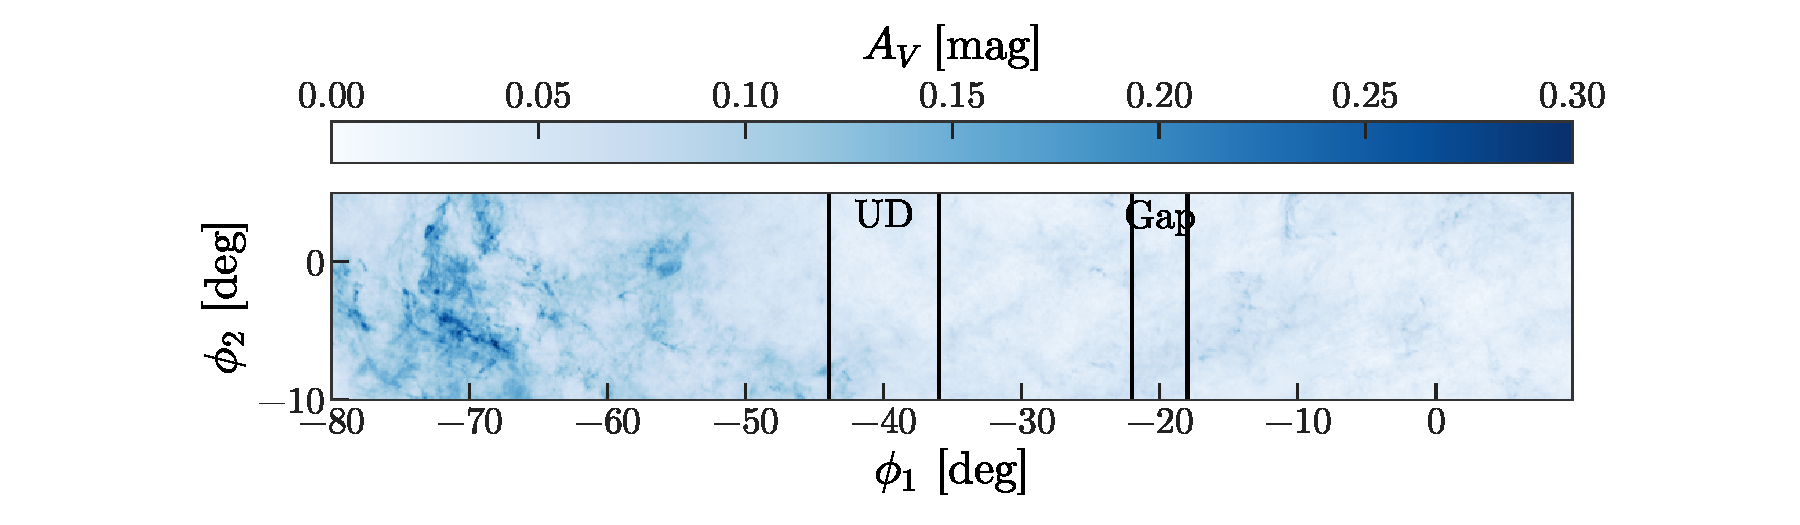
\includegraphics[width=\textwidth]{sfd.pdf}
\end{center}
\caption{%
Colored background shows the $V$-band extinction, $A_V$, in the GD-1
coordinate system.
Vertical lines roughly show the extents the identified under-density (UD) and
gap.
The maximum extinction in the UD or Gap regions is $\approx$0.07 mag.
\label{fig:sfd}
}
\end{figure}


\section{Results}
\label{sec:results}

\subsection{Global properties}
\label{sec:res_global}

\subsection{Gap}
\label{sec:res_gap}

\subsection{Underdensity}
\label{sec:res_underdensity}


\section{Discussion}
\label{sec:discussion}


\acknowledgements{
Gaia
Belokurov, Casey, Geha, Hogg, Johnston, Koposov, Lisanti, Schlafly, Spergel
This research was started at the NYC Gaia DR2 Workshop at the Center for Computational Astrophysics of the Flatiron Institute in 2018 April.
AB acknowledges generous support from the Institute for Theory and Computation at Harvard University.
All code used in this work and all results are available at \url{https://github.com/adrn/GD1-DR2}.
}

\software{
    \package{Astropy} \citep{astropy},
    \package{dustmaps}\footnote{\url{https://github.com/gregreen/dustmaps}},
    \package{gala} \citep{gala},
    \package{IPython} \citep{ipython},
    \package{matplotlib} \citep{mpl},
    \package{numpy} \citep{numpy},
    \package{scipy} \citep{scipy}
}

\bibliographystyle{aasjournal}
\bibliography{gd1}

\clearpage

\appendix
\section{Completeness check and data validation}
\label{sec:validate}

% % Notebook:
% \begin{figure}[h]
% \begin{center}
% \includegraphics[width=0.7\textwidth]{nvisits.pdf}
% \end{center}
% \caption{%
% TODO
% \label{fig:TODO}
% }
% \end{figure}


\end{document}
